\documentclass[12pt,letterpaper]{article}
\usepackage{fullpage}
\usepackage[top=2cm, bottom=4.5cm, left=1.5cm, right=1.5cm]{geometry}
\usepackage{amsmath,amsthm,amsfonts,amssymb,amscd}
\usepackage{lastpage}
\usepackage{enumerate}
\usepackage{fancyhdr}
\usepackage{mathrsfs}
\usepackage{xcolor}
\usepackage{graphicx}
\usepackage{float}
\usepackage{subfigure}
\usepackage{listings}
\usepackage{hyperref}
\usepackage{mathtools}
\usepackage{xfrac}
\usepackage{bbm}

\hypersetup{
  colorlinks=true,
  linkcolor=blue,
  linkbordercolor={0 0 1}
}
\linespread{1.1}
 
\renewcommand\lstlistingname{Algorithm}
\renewcommand\lstlistlistingname{Algorithms}
\def\lstlistingautorefname{Alg.}


\lstdefinestyle{Python}{
    language        = Python,
    frame           = lines, 
    basicstyle      = \footnotesize,
    keywordstyle    = \color{blue},
    stringstyle     = \color{green},
    commentstyle    = \color{red}\ttfamily
}

\setlength{\parindent}{0.0in}
\setlength{\parskip}{0.05in}

\newcommand\course{Computer Vision}
\newcommand\hwnumber{1}
\newcommand\NetIDa{SUN Yilin}
\newcommand\NetIDb{520030910361}

\pagestyle{fancyplain}
\headheight 35pt
\lhead{\NetIDa}
\lhead{\NetIDa\\\NetIDb}
\chead{\textbf{\Large Homework \hwnumber}}
\rhead{\course \\ \today}
\lfoot{}
\cfoot{}
\rfoot{\small\thepage}
\headsep 1.5em

\begin{document}

\section{Written Assignment}
\subsection*{a}
The shape of the image will still be a circular disk, with different radius.\\
\textbf{Explanations:}
We use the same setting as our lecture notes, i.e. $\boldsymbol{r_o}=(x_o,y_o,z_o)$ denotes
the coordinate of actual object pixel and $\boldsymbol{r_i}=(x_i,y_i,f)$ denotes its image.
We set the pinhole $(x,y,z)=(0,0,0)$ and let the optical axis be the $z$-axis.
Now we prove our argument by deriving the equation of the image of the disk.\\
The equation of the circular disk in original space can be described as $(x_o-a)^2+(y_o-b)^2=c^2$
where $(a,b)$ is its center and $c$ is its radius. Then by applying the rule of similar triangles 
we get $(x_i,y_i)=(\frac{fx_o}{z_o},\frac{fy_o}{z_o})$, then by substituting the coordinates
we get the equation of image disk as $(\frac{z_ox_i}{f}-a)^2+(\frac{z_oy_i}{f}-b)^2=c^2$,
or equivalently $$(x_i-\frac{af}{z_o})^2+(y_i-\frac{bf}{z_o})=(\frac{cf}{z_o})^2$$
which is still a circular disk in image plane.
\subsection*{b}
\textbf{Case 1:} plane $y=0$\\
The direction vectors on this plane can be expressed generally as $(x_i,0,z_i)$.
Then the vanishing points of the family of lines represented by these family of vectors
can be expressed as $(f\frac{x_i}{z_i},0)$ by our formula from lecture slides.
Then we know the vanishing points $(f\frac{x_i}{z_i})$ actual lie on line $y=0$ in the image plane.\\
\textbf{Case 2:} plane $x=0$\\
Now the direction vectors are $(0,y_i,z_i)$ and the vanishing points are $(0,f\frac{y_i}{z_i})$.
This time the vanishing points lie on the line $x=0$ in the image plane.
\subsection*{c}
Generally, the normal vector of plane $Ax+By+Cz+D=0$ is $(A,B,C)$, thus any direction vector $(x_i,y_i,z_i)$
that lies in this plane must satisfy that $Ax_i+By_i+Cz_i=0$. 
Then we know that the vanishing point of line $(x_i,y_i,z_i)$ is $(f\frac{x_i}{z_i},f\frac{y_i}{z_i})$.
(Note that $z_i$ cannot be zero, otherwise there will not be a vanishing point for these lines parallel to the image plane)\\
These vanishing points $(f\frac{x_i}{z_i},f\frac{y_i}{z_i})$ actually lie on line
$$Ax+By+Cf=0$$

\newpage
\section{Programming Assignment}

\subsection{}
\subsubsection*{a}
I use the default threshhold value 128.\\
The function is straightforward. It takes the gray image as input and do an element-wise operation 
to set all those values larger than threshhold value as 255, 
meanwhile other values remain zero.
\begin{figure}[htbp]
  \centering
  \subfigure[two\_objects]{
  \label{bintwo}
  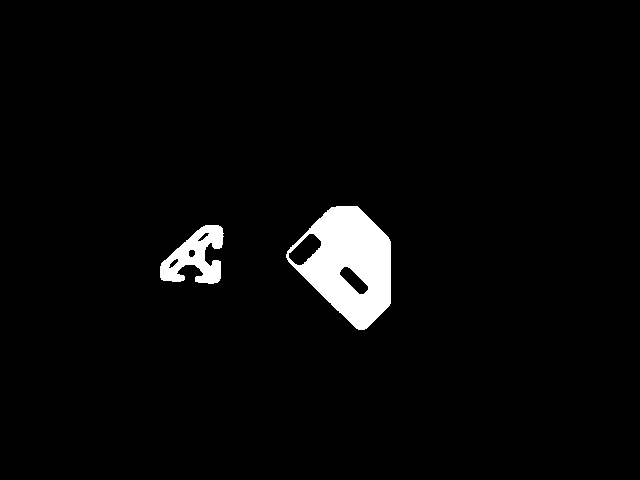
\includegraphics[width=0.3\textwidth]{../output/two_objects_binary.png}}
  \subfigure[many\_objects\_1]{
  \label{binmany1}
  
\includegraphics[width=0.325\textwidth]{../output/many_objects_1_binary.png}}
  \subfigure[many\_objects\_2]{
  \label{binmany2}
  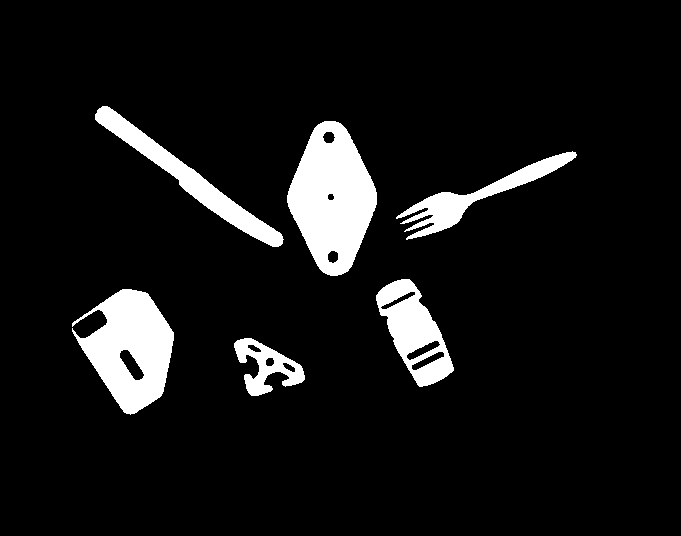
\includegraphics[width=0.325\textwidth]{../output/many_objects_2_binary.png}}
  \caption{binary images of various input}
  \label{binary_img}
\end{figure}

\subsubsection*{b}
I implemented the sequential labeling algorithm by making two passes of the image.
In the first pass I label all those connected components by scanning the array from
top to down and from left two right. 
Meanwhile I used the union-find-set data structure to mark the equivalent classes.
In the second pass I merge the equivalent classes, calculate the number of total connected components 
and mark them with different gray levels by a normalization over interval [0,255].
\begin{figure}[htbp]
  \centering
  \subfigure[two\_objects]{
  \label{labtwo}
  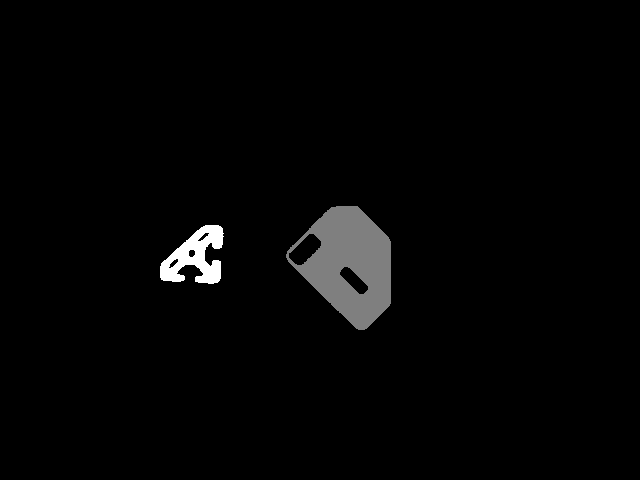
\includegraphics[width=0.3\textwidth]{../output/two_objects_labeled.png}}
  \subfigure[many\_objects\_1]{
  \label{labmany1}
  
\includegraphics[width=0.325\textwidth]{../output/many_objects_1_labeled.png}}
  \subfigure[many\_objects\_2]{
  \label{labmany2}
  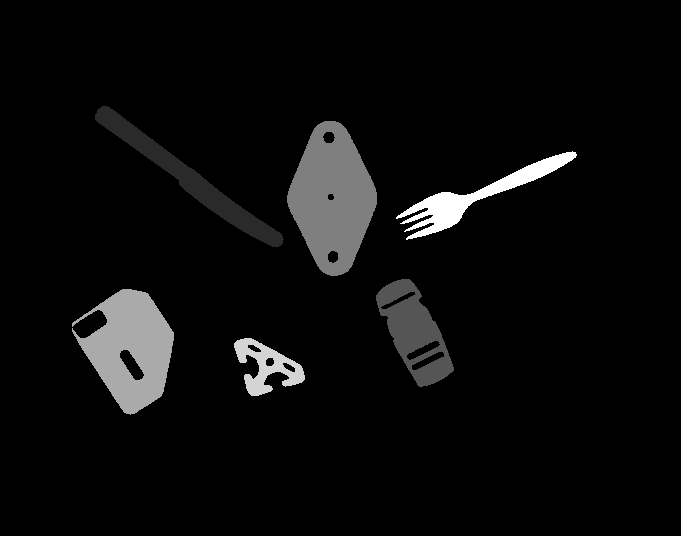
\includegraphics[width=0.325\textwidth]{../output/many_objects_2_labeled.png}}
  \caption{labeled images of various input}
  \label{labeled_img}
\end{figure}

\subsubsection*{c}
This function is simply the implementation of the formulas given in our lecture notes.
The results on various images are listed below. 
\begin{figure}[htbp]
  \centering
  \includegraphics[scale=0.48]{../output/attributes.png}
  \label{att}
  \caption{attributes of various images}
\end{figure}

\subsection{}
\subsubsection*{a}
The Sobel mask is equivalent to what we defined in class, i.e.
$$Sobel_{x}=
\begin{pmatrix}
  -1 & 0 & 1\\
  -2 & 0 & 2\\
  -1 & 0 & 1
\end{pmatrix} \qquad
Sobel_{y}=
\begin{pmatrix}
  1 & 2 & 1\\
  0 & 0 & 0\\
  -1 & -2 & -1
\end{pmatrix}
$$
I then implement convolution operation and finish the edge detect operation.
\subsubsection*{b}
I choose edge threshhold value 140 and \{24,25,\dots,30\} as possible radius values.

\subsubsection*{c}
The maximum intensity of my accumulation array is about 106,
after careful examination, I choose hough threshold value as 75.
At this threshold, we are able to detect all the circles at a fast speed.
Also I used the NMS operation to filter out multiple circles centerd at the same point.\\
The circle parameters given as a list of tuple are:\\
(29, 105, 34)(24, 49, 55)(29, 145, 94)(24, 84, 109)(29, 207, 118)\\
(28, 33, 146)(29, 118, 173)(28, 69, 215)(24, 172, 234)(24, 101, 263)
\begin{figure}[htbp]
  \centering
  \subfigure[edge intensity]{
  \label{edgeintense}
  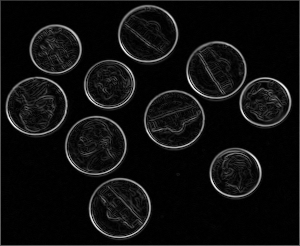
\includegraphics[width=0.32\textwidth]{../output/coins_normalized_edges.png}}
  \subfigure[edge threshholded]{
  \label{edgethresh}
  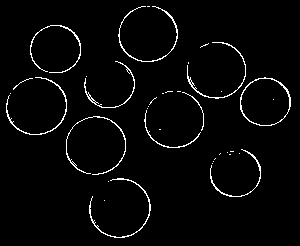
\includegraphics[width=0.32\textwidth]{../output/coins_edges.png}}
  \subfigure[circles with NMS operation]{
  \label{drawcircle}
  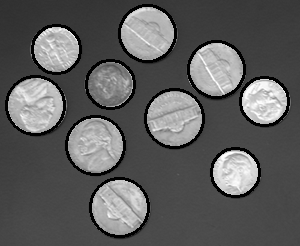
\includegraphics[width=0.32\textwidth]{../output/coins_circles.png}}
  \caption{Results of problem 2}
  \label{labeled_img}
\end{figure}

\end{document}